\documentclass[twoside]{protokoll}
\usepackage{graphicx}
\usepackage{tabularx}
\usepackage{booktabs}
\usepackage{float} 
\praktikum{I}
\usepackage{subfig}
\usepackage{amsmath}

\versuchsgebiet{(Mechanik)}


\teilnehmer{Maximilian Carlos Menke, 434170}
\teilnehmer{Andrea Roth, 428396}
\gruppe{A3}

\begin{document}
 
%TODO check section name
\section{1M1 Messung der Erdbeschleunigung mit dem Pendel}
\begin{figure}[H]
    \centering
    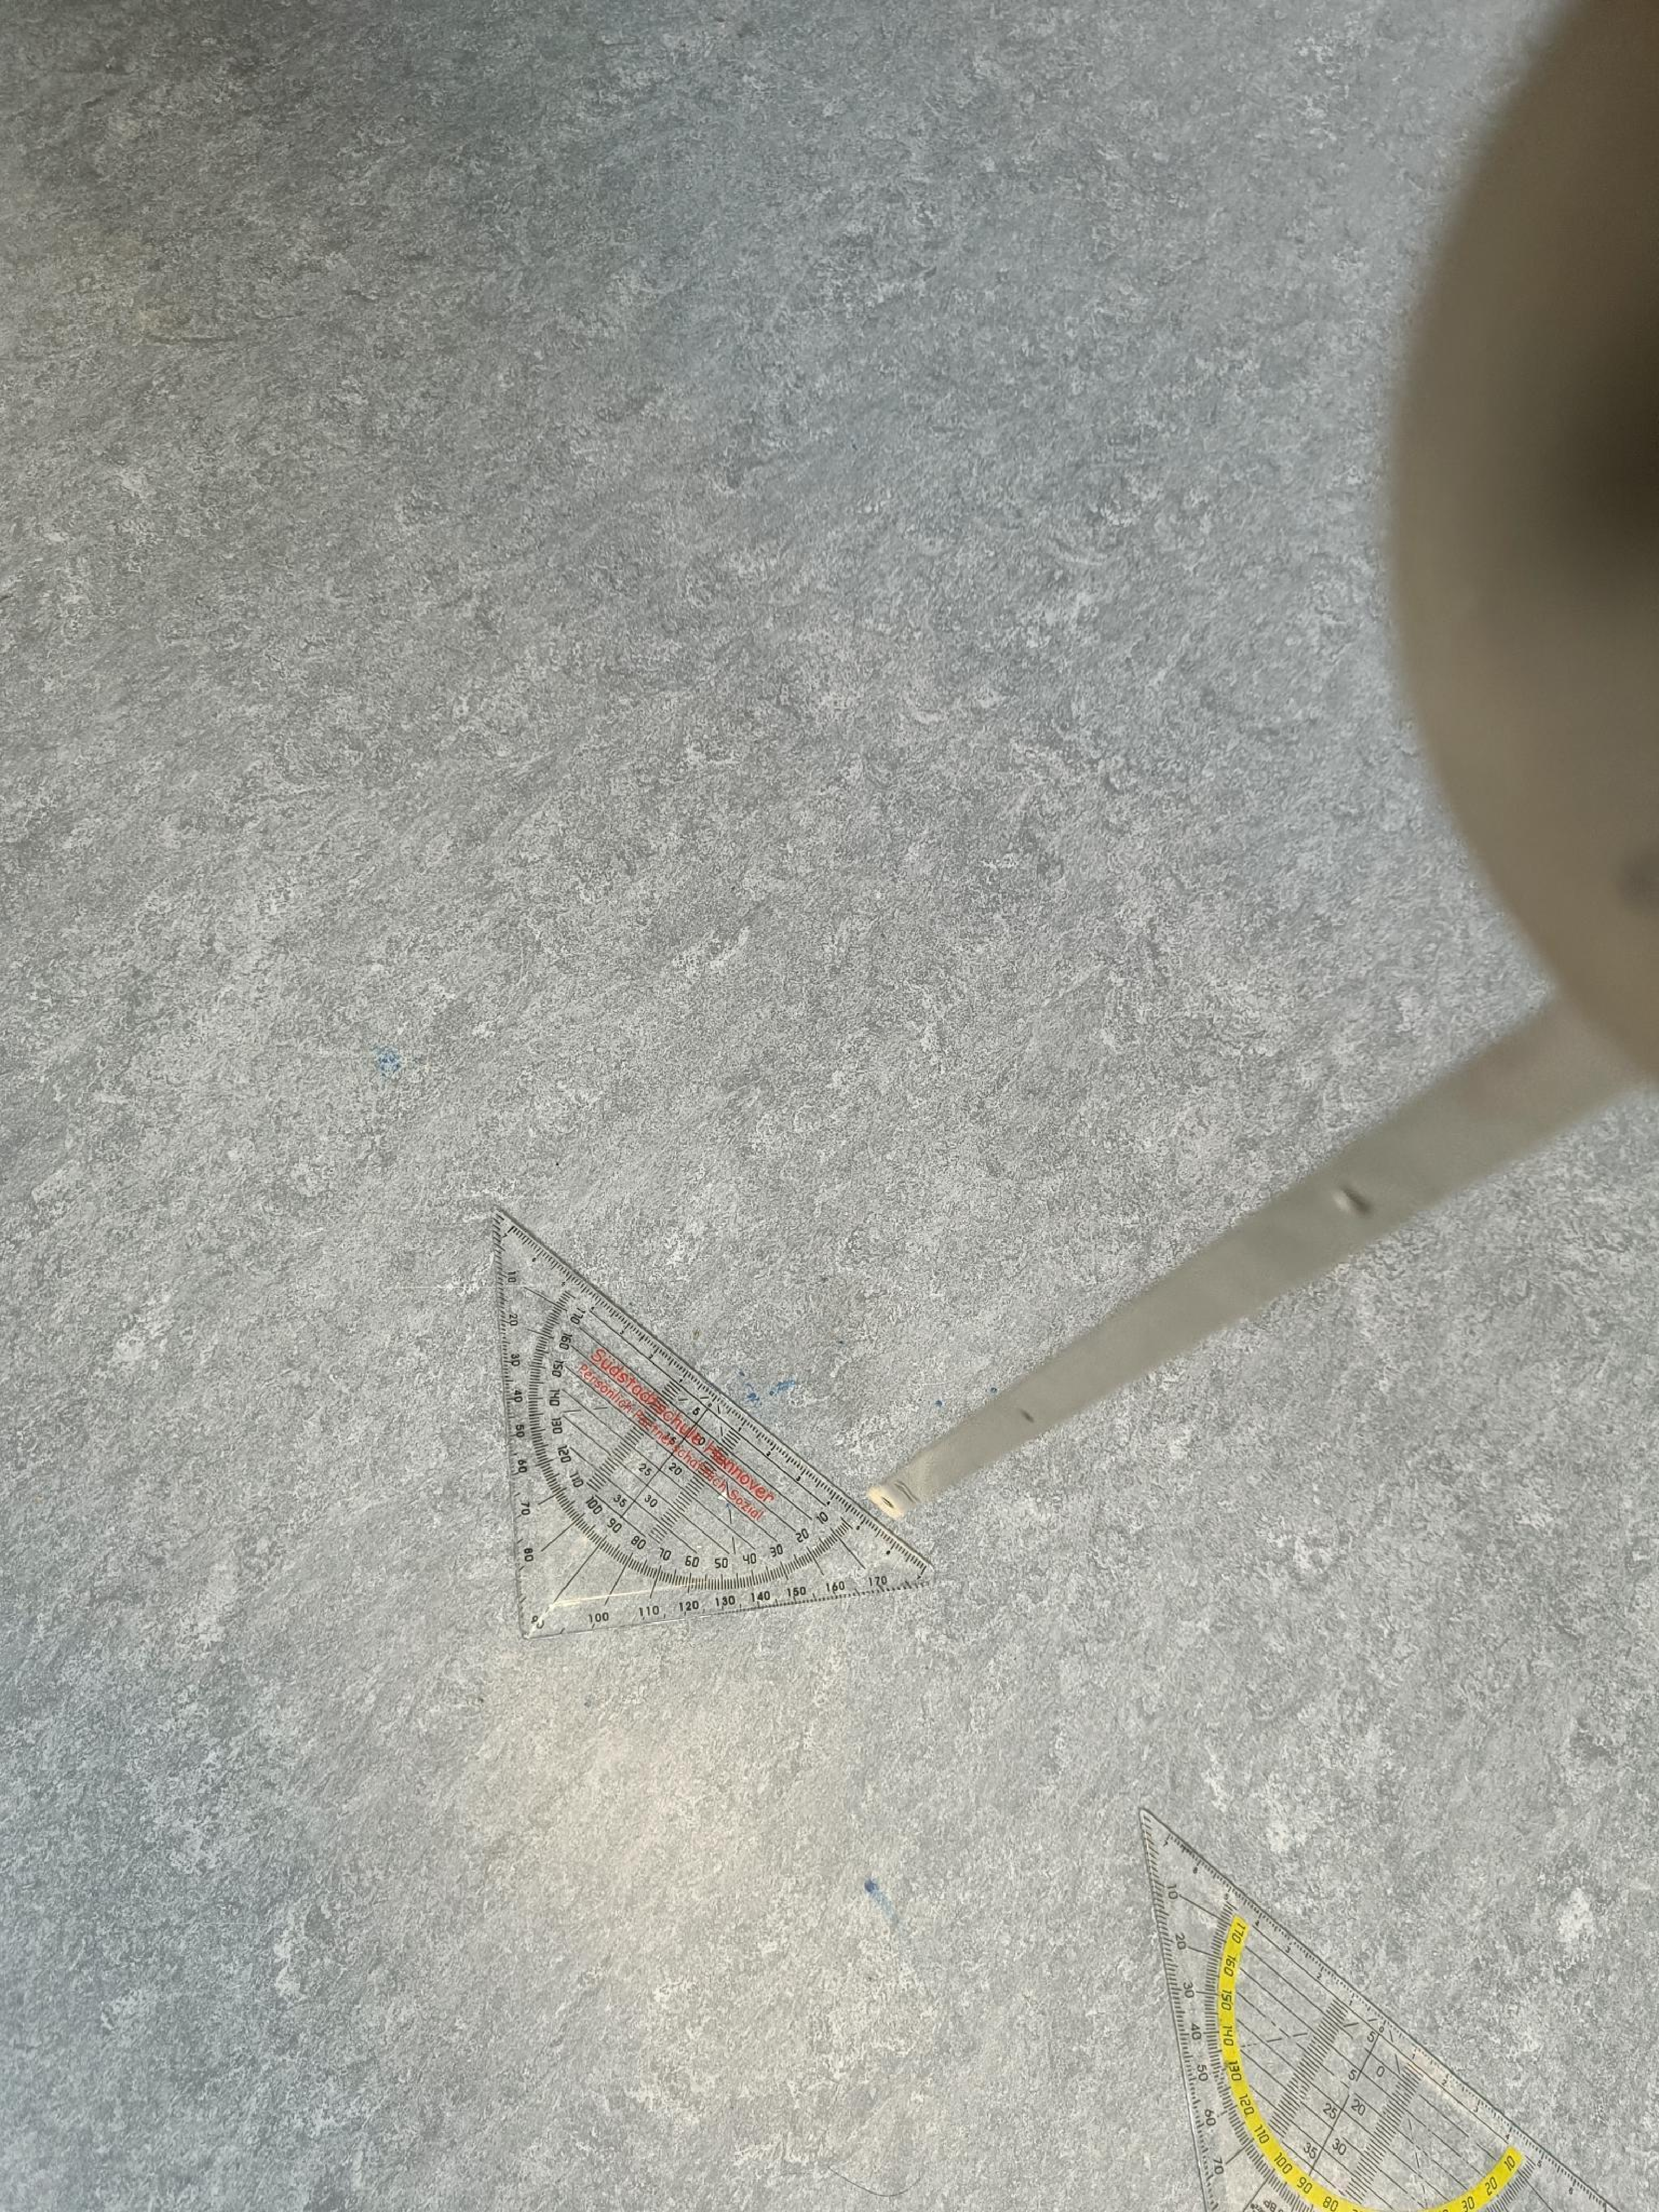
\includegraphics[width=0.5\textwidth]{Bilder/signal-2023-03-22-155329_002.pdf}
    \caption{Schwingkreis 1}
    \label{fig:Schwingkreis1}
\end{figure}

\begin{aufgabe}{Grundlagen}
  Knappe Beschreibung der theoretischen Grundlagen, Angabe der
  benötigten Formel(n), ohne Herleitung. Definition der verwendeten
  Formelzeichen.
\end{aufgabe}

Ein Pendel kann als physikalischens Pendel beschrieben werden.
Dabei wirkt auf das Pendel eine Kraft von $F_g = m_S \cdot g$, wobei $g$ die zu bestimmende Erdbeschleunigung ist und $m_S$ die Schwere Masse des Pendels.
Beim Schwingen, befindet sich das Pendel oftmals nicht in der Ruhelage, sondern ist in einer Auslenkung $\varphi$ vom Gleichgewichtszustand entfernt.
Dann wirkt ein rückstellendes Drehmoment $ M = l \cdot F_r$ (mit $l$ als Länge von der Rotations Achse zum Schwerpunkt).
Da unser Pendel Träge ist, entsteht eine Schwingung: 
\begin{equation}
    J \cdot \ddot{\varphi} = -m \cdot g \cdot l^2 \cdot \sin(\varphi)
\end{equation}
Dabei verwenden wir im Folgenden die Kleinwinkel näherung $\sin(\varphi) \approx \varphi$.
Diese gilt für Auslenkungen von weniger als $5$°. Damit lässt sich die Bewegungsgleichung vereinfachen:
\begin{equation}
    J \cdot \ddot{\varphi} \approx -m \cdot g \cdot l^2 \cdot \varphi
\end{equation}
Das Trägheitsmoment ist dabei wie folgt definiert:
\begin{equation}
    J =  m_T \cdot l^2
\end{equation}
Hierbei ist $m_T$ die Träge Masse des Pendels. Dies ist nach dem Einsteinischen Äquivalenzprinzip aber gleich der schweren Masse, und somit $m_T = m$.
Aufgelöst nach $\ddot{\varphi}$ ergibt sich ( mit $\omega$ als Winkelgeschwindigkeit der Schwingung):
\begin{equation}
    \ddot{\varphi} \approx -\frac{g}{l} \cdot \varphi = - \omega^2 \cdot \varphi
\end{equation}
Aus dieser DGL lässt sich $\varphi(t)$ bestimmen, zu:
\begin{equation}
    \varphi(t) = \varphi_{max} \cdot \cos(\omega \cdot t)
\end{equation}
Daraus ergibt sich (mit $T$ als dauer einer Schwingungsperiode):
\begin{equation}
    \omega^2 = \frac{m \cdot g \cdot l_s}{J}
\end{equation}
\begin{equation}
    \Rightarrow T = \frac{1}{g} 4 \cdot \pi^2 \cdot \frac{J}{m l_s}
\end{equation}
Dabei kann man $\omega$ als Quotient von rückstellendem Drehmoment und Trägheitsmoment beschreiben.
Hier sind alle Größen mit einem einem G versehen sind dem Gewicht zugehörig. Die mit einem $_st$ versehnen Größen gehören nur zur Stange.
\begin{equation}
    \omega_{st}^2 = \frac{M_{st}}{J_{st}}
\end{equation}
\begin{equation}
    \omega_{G}^2 = \frac{M_G}{J_G}
\end{equation}
Wenn man die Position des Gewichtes so einstellt, dass die Schwingung der Stange die gleiche Periodendauer hat wie die Schwingung des Gewichtes, dann gilt:
\begin{equation}
    \omega_{st}^2 = \omega_{G}^2
\end{equation}
\begin{equation}
    \omega^2 = \frac{M_{st}}{J_{st}} = \frac{M_G}{J_G}
\end{equation}
Das bedeutet das wir das Pendel mit Gewicht so behandeln können, als wäre es an einer Massefreihen Stange aufgehangen.




\begin{aufgabe}{Versuchsaufbau und Versuchsdurchführung}
  Beschreibung des Versuchsaufbaus einschließlich beschrifteter Skizze
  oder Foto. Beschreibung der Versuchsdurchführung: Handgriffe an der
  Apparatur, verwendete Messwerterfassungseinstellungen, Messbereiche,
  Triggerbedingungen, etc.
\end{aufgabe}

Kurz zusammengefasst besteht der Versuchsaufbau aus einem Stabilen dreieckigen Stativ, an welchem ein Winkelaufnehmer befestigt wird.
An diesen Winkelaufnehmer Wird ein Pendel gehangen, welches aus einem U-Profil, mit zwei Metallnadeln als Aufhängung, einer flachen Pendelstange, und einem Pendelkörper besteht.\\


Der Oberen Skizze kann der Gesamtaufbau entnommen werden. 
Zunächst werden zwei Tischklemmen mit je einer Stativ Stange am vorne Tisch befestigt.
Die dritte Stativ Stange wird auf der anderen Seite des Tisches in der bereits angebrachten Halterung befestigt. 
Mit Kreuzmuffen werden nun die langen Metallstangen verwendet um diese 3 Stativ Stangen zu verbinden, und so ein Dreieck zu bilden.
Es sollte darauf geachtet, werden, das die Stangen gut in den Kreuzmuffen liegen. 
Bei der vorderen Stange an welcher später das Pendel auf gehangen wird, muss darauf geachtet werden, dass diese horizontal ist.
Dies kann mithilfe der Wasserwaage überprüft werden.\\

Wenn diese Konstruktion stabil ist, kann vorne an der Stange der Winkelaufnehmer befestigt werden. 
Dieser besteht aus einer Stange in welcher 2 Nut sind mit eine Hall-Sonde. 
Dies wird an das CASSY angeschlossen.
Wir haben beide Winkelaufnehmer befestigt, um zu überprüfen welchen wir besser Nullen können, und damit wir später ein Pendel mit und eins ohne Pendelkörper bei der Synchronisation vergleichen können.
Bei den Winkelaufnehmern muss darauf geachtet werden, dass diese fest genug befestigt sind, sodass sich diese nicht verdrehen bei dem Pendelvorgang.\\

Die beide Pendelstangen werden an ein U-Profil geschraubt.
Das U-Profil besteht aus zwei Permanentmagneten die ein homogenes Magnetfeld um die Hall-Sonde erzeugen, Zwei Nadeln auf denen das Pendel schwingen wird, und einer Halterung für die Stange. 
Die zwei Nadeln, werden in die Nut an dem Winkelaufnehmer gestellt.
Der Stellpunkt der Nadeln ist die Rotationsachse des der Pendelschwingung. \\

Ein Pendelkörper kann an der Pendelstange befestigt werden, indem man die Stange in diesen schiebt, und mit der Schraube des Pendelkörpers festzieht. 


\begin{aufgabe}{Rohdaten}
  Stellen Sie Ihre Rohdaten dar, tabellarisch für $l_p$ und $r_p$,
  grafisch für den Verlauf der Schwingung der Stange ohne Pendelkörper
  sowie der Pendelschwingung (für mindestens drei Messreihen).
\end{aufgabe}


\begin{aufgabe}{Auswertung}
  Bestimmen Sie für alle Messreihen die Periodendauer und ihre
  Messunsicherheit, indem Sie eine geeignete lineare Regression
  durchführen. Demonstrieren Sie, dass Sie das Trägheitsmoment der
  Stange kompensiert haben. Tabellieren Sie die Zwischenergebnisse
  der relevanten Größen samt ihrer Messunsicherheiten. Berechnen
  Sie die Erdbeschleunigung. Führen Sie eine Fehlerrechnung zur
  Bestimmung der Messunsicherheit durch. Geben Sie bei Ihrer
  Fehlerrechnung die Größe der Einzelbeiträge an, die zu dem
  Gesamtfehler führen. Diskutieren Sie, welcher Fehler den
  Gesamtfehler dominiert. Vergleichen Sie Ihr Endergebnis mit dem
  relevanten Literaturwert.
\end{aufgabe}

\end{document}
